\subsection{Learning denoised representations}
\label{hsicdenoise}
This section presents a case study of denoising datasets in the setting of an important open scientific problem. The task of \emph{denoising} consists of representing experimental observations $x$ and nuisance observations $s$ with two independent signals: biological signal $z$ and technical noise $u$. The difficulty is that $x$ contains both biological signal and noise and is therefore strongly correlated with $s$ (Figure~\ref{hsicpgm}c). In particular, we focus on single-cell RNA sequencing (scRNA-seq) data which renders a gene-expression snapshot of an heterogeneous sample of cells. Such data can reveal a cell's type~\cite{Wagner2016, Tanay2017}, if we can cope with a high level of technical noise~\cite{Grun2014}.


\subsubsection{Data presentation}
The output of an scRNA-seq experiment is a list of transcripts $(l_m)_{m \in \mathcal{M}}$. Each transcript $l_m$ is an mRNA molecule enriched with a cell-specific barcode and a unique molecule identifier, as in \cite{Klein2015}. Cell-specific barcodes enable the biologist to work at single-cell resolution. Unique molecule identifiers (UMIs) are meant to remove some significant part of the technical bias (e.g., amplification bias) and make it possible to obtain an accurate probabilistic model for these datasets~\cite{Lopez292037}. Transcripts are then aligned to a reference genome with tools such as CellRanger~\cite{Zheng2017}.

The data from the experiment has two parts. First, there is a gene expression matrix $(X_{ng})_{(n, g) \in \mathcal{N}\times\mathcal{G}}$, where $\mathcal{N}$ designates the set of cells detected in the experiment and $\mathcal{G}$ is the set of genes the transcripts have been aligned with. A particular entry of this matrix indicates the number of times a particular gene has been expressed in a particular cell. Second, we have quality control metrics $(s^i)_{i\in \mathcal{S}}$ which assess the level of errors and corrections in the alignment process:
\begin{itemize}
\item $s^1$: proportion of transcripts which confidently mapped to a gene;
\item $s^2$: proportion of transcripts mapping to the genome, but not to a gene;
\item $s^3$: proportion of transcripts which did not align;
\item $s^4$: proportion of transcripts whose UMI sequence was corrected by the alignment procedure;
\item $s^5$:~proportion of transcripts whose barcode sequence was corrected by the alignment procedure.
\end{itemize}
These metrics cannot be described with a generative model as easily as gene expression data but they nonetheless impact a significant number of tasks in the research area~\cite{Cole2017}. Another significant portion of these metrics focus on the sampling effects (i.e., the discrepancy in the total number of transcripts captured in each cell) which can be taken into account in a principled way in a graphical model as in~\cite{Lopez292037}. 

\begin{figure}[h!]

    
    
      \tikzstyle{latent} = [circle,fill=white,draw=black,inner sep=1pt,
minimum size=30pt, font=\fontsize{15}{15}\selectfont, node distance=1]


  \newcommand{\ltkiz}{1cm}
  
  
\captionsetup[subfigure]{justification=centering}
    \centering  
    \begin{subfigure}[t]{0.3\textwidth}
        \centering   
		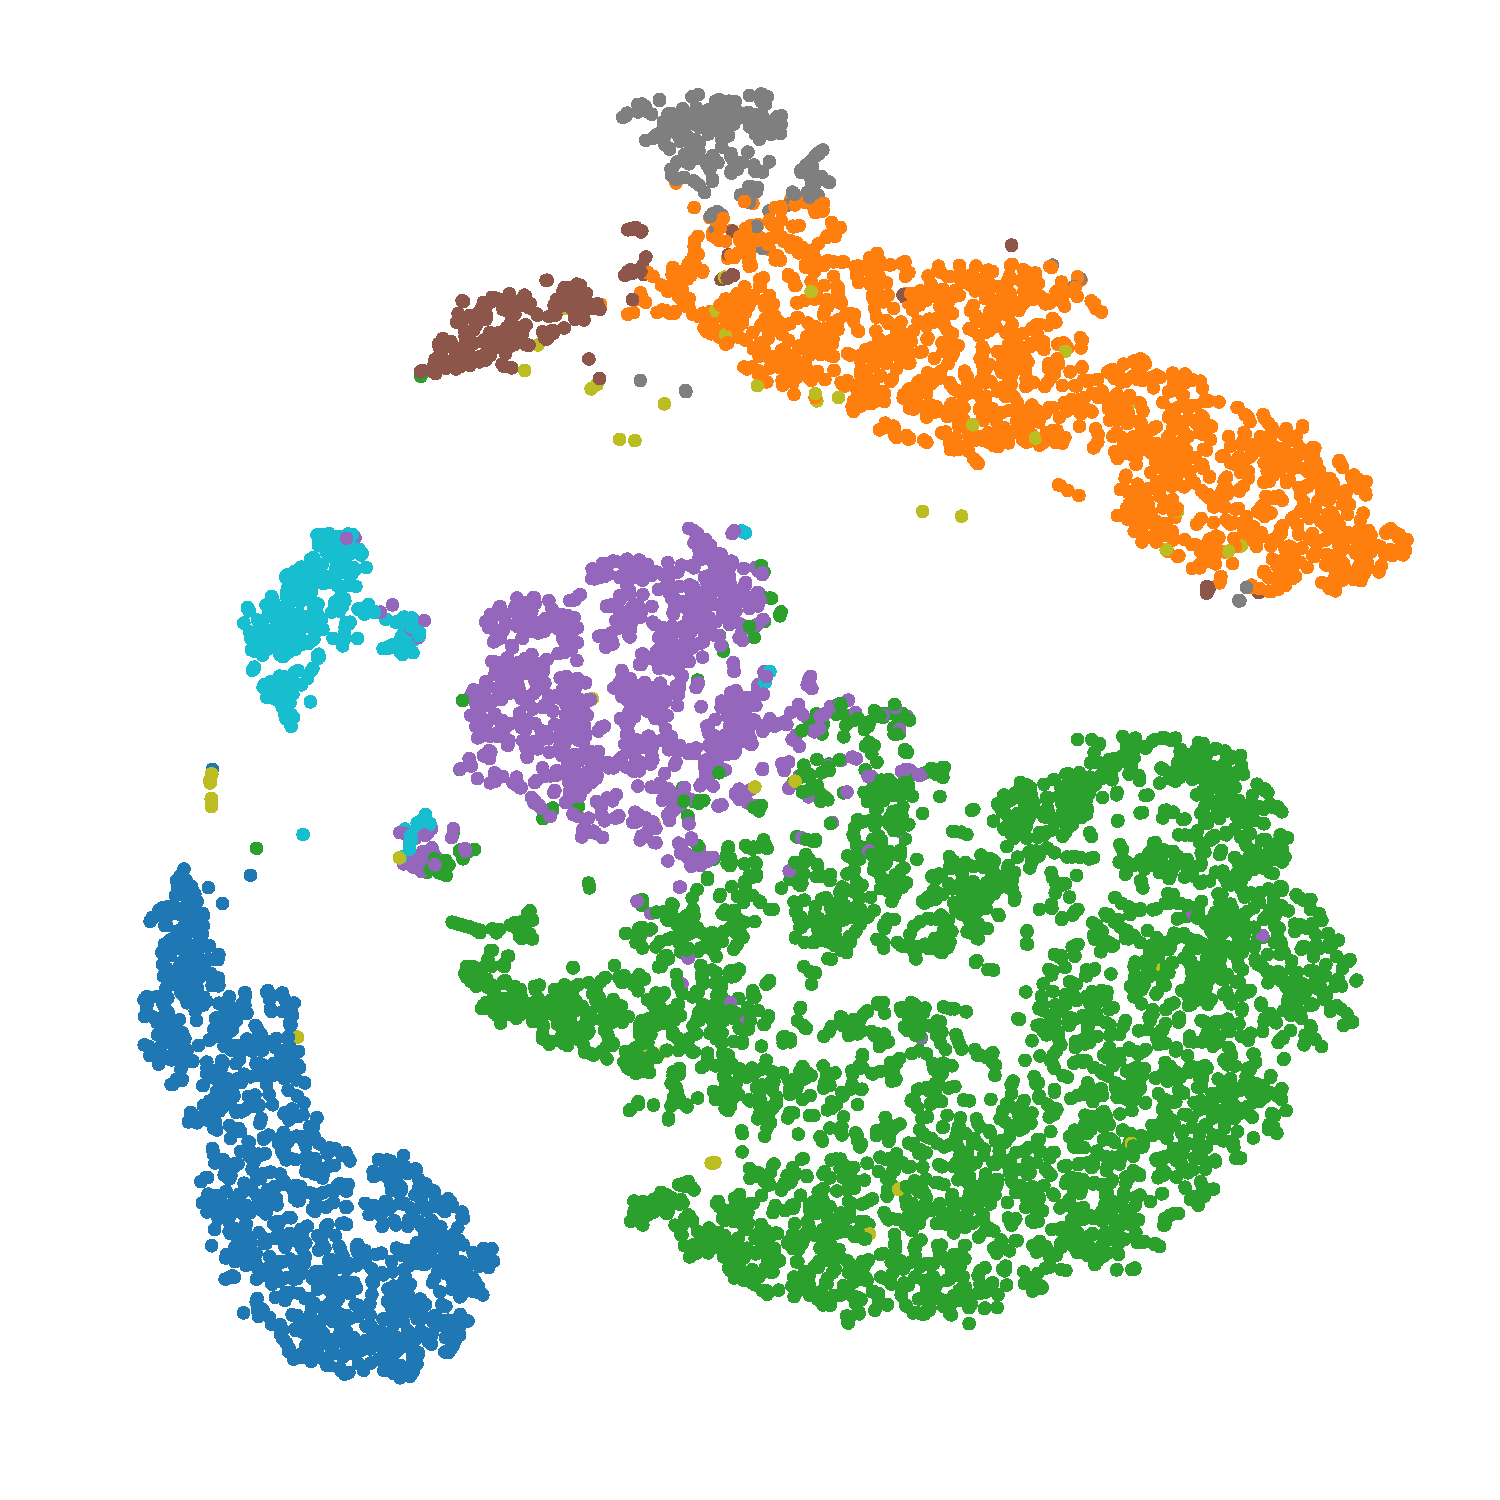
\includegraphics[width=3.5cm]{figures/cell_types.pdf}
        \caption{Embedding of $x$: gene expression data. Each point is a cell. Colors are cell-types.}
    \end{subfigure}%
    ~  
    \begin{subfigure}[t]{0.3\textwidth}
        \centering  
		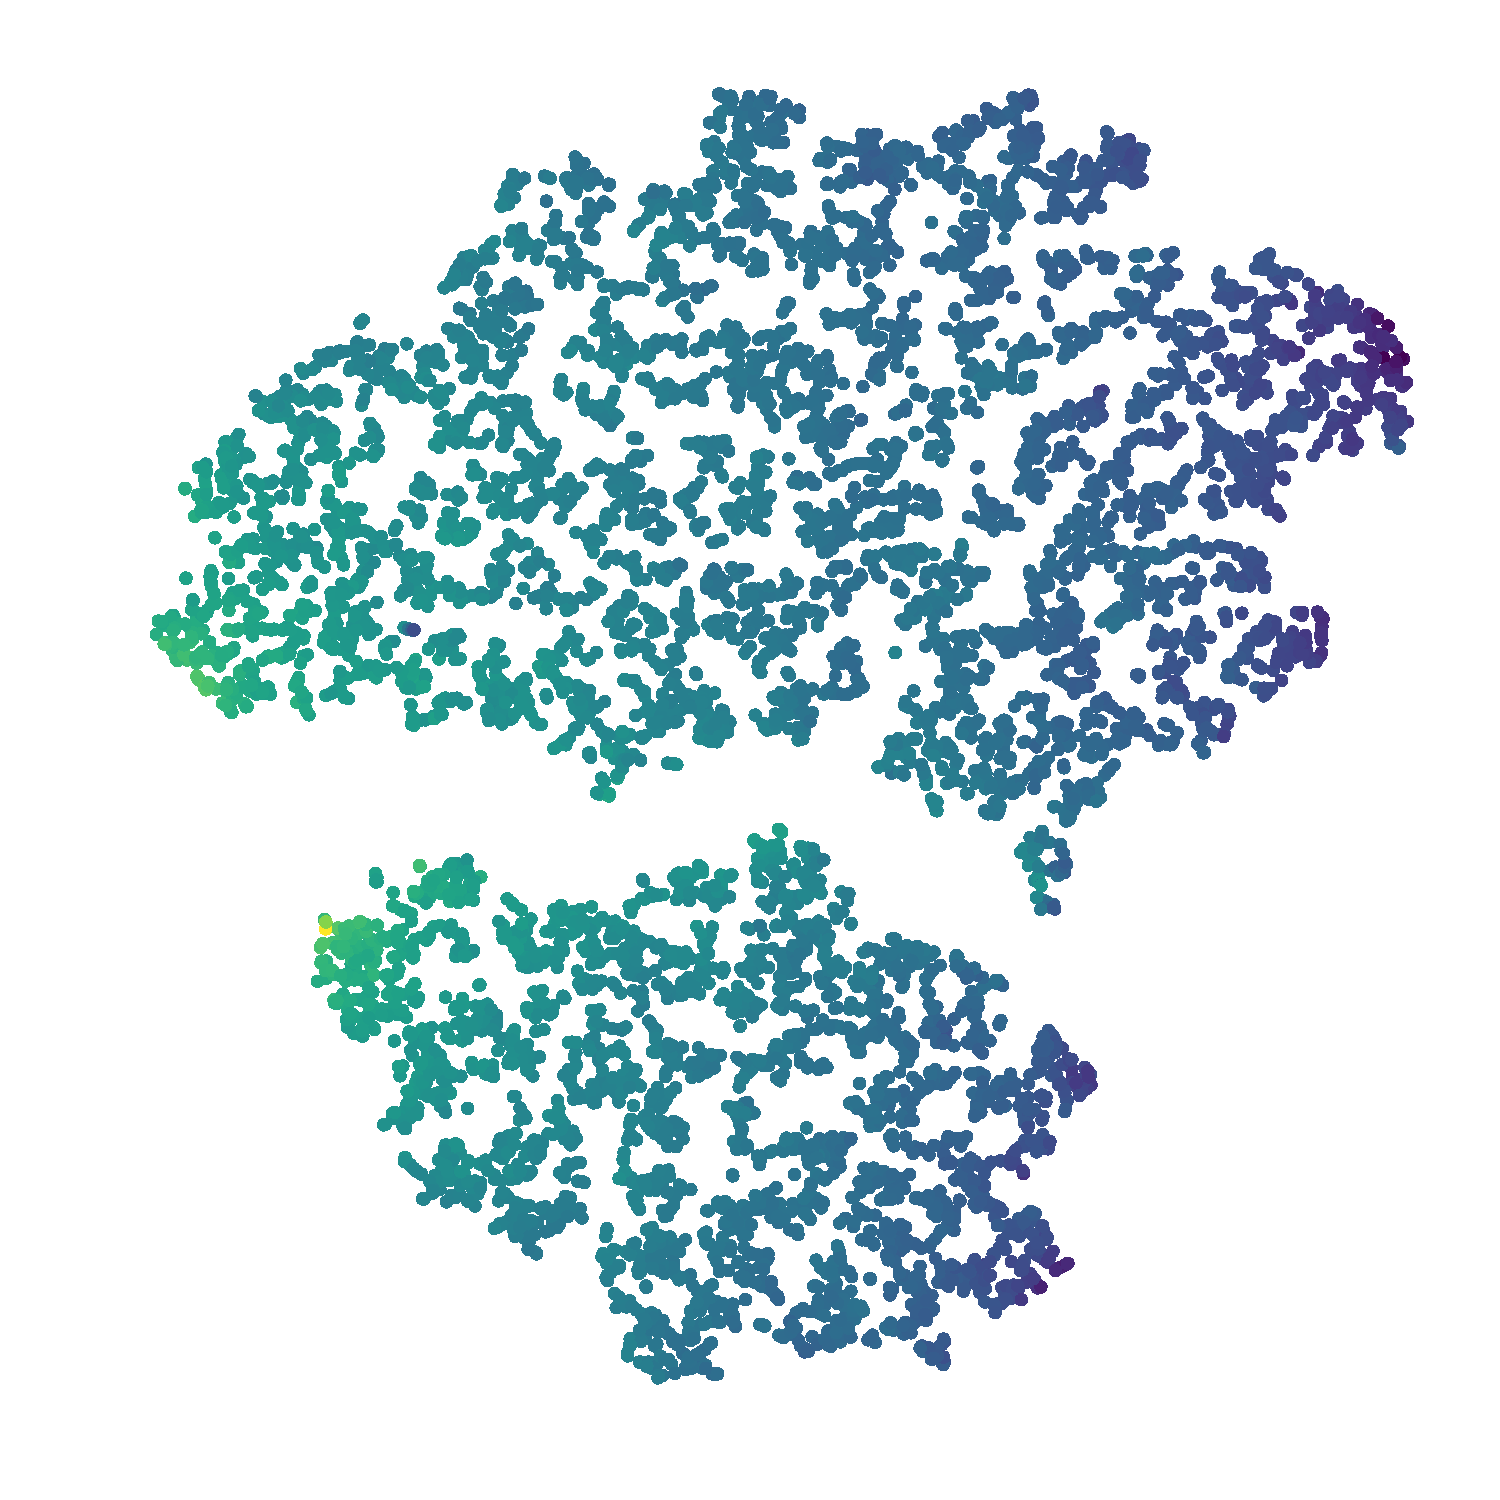
\includegraphics[width=0.7\textwidth]{figures/qc.pdf}
        \caption{Embedding of $s$: alignment errors. Each point is a cell. Color is $s^1$.}
    \end{subfigure}
    ~
    \begin{subfigure}[t]{0.3\textwidth}
        \centering  
		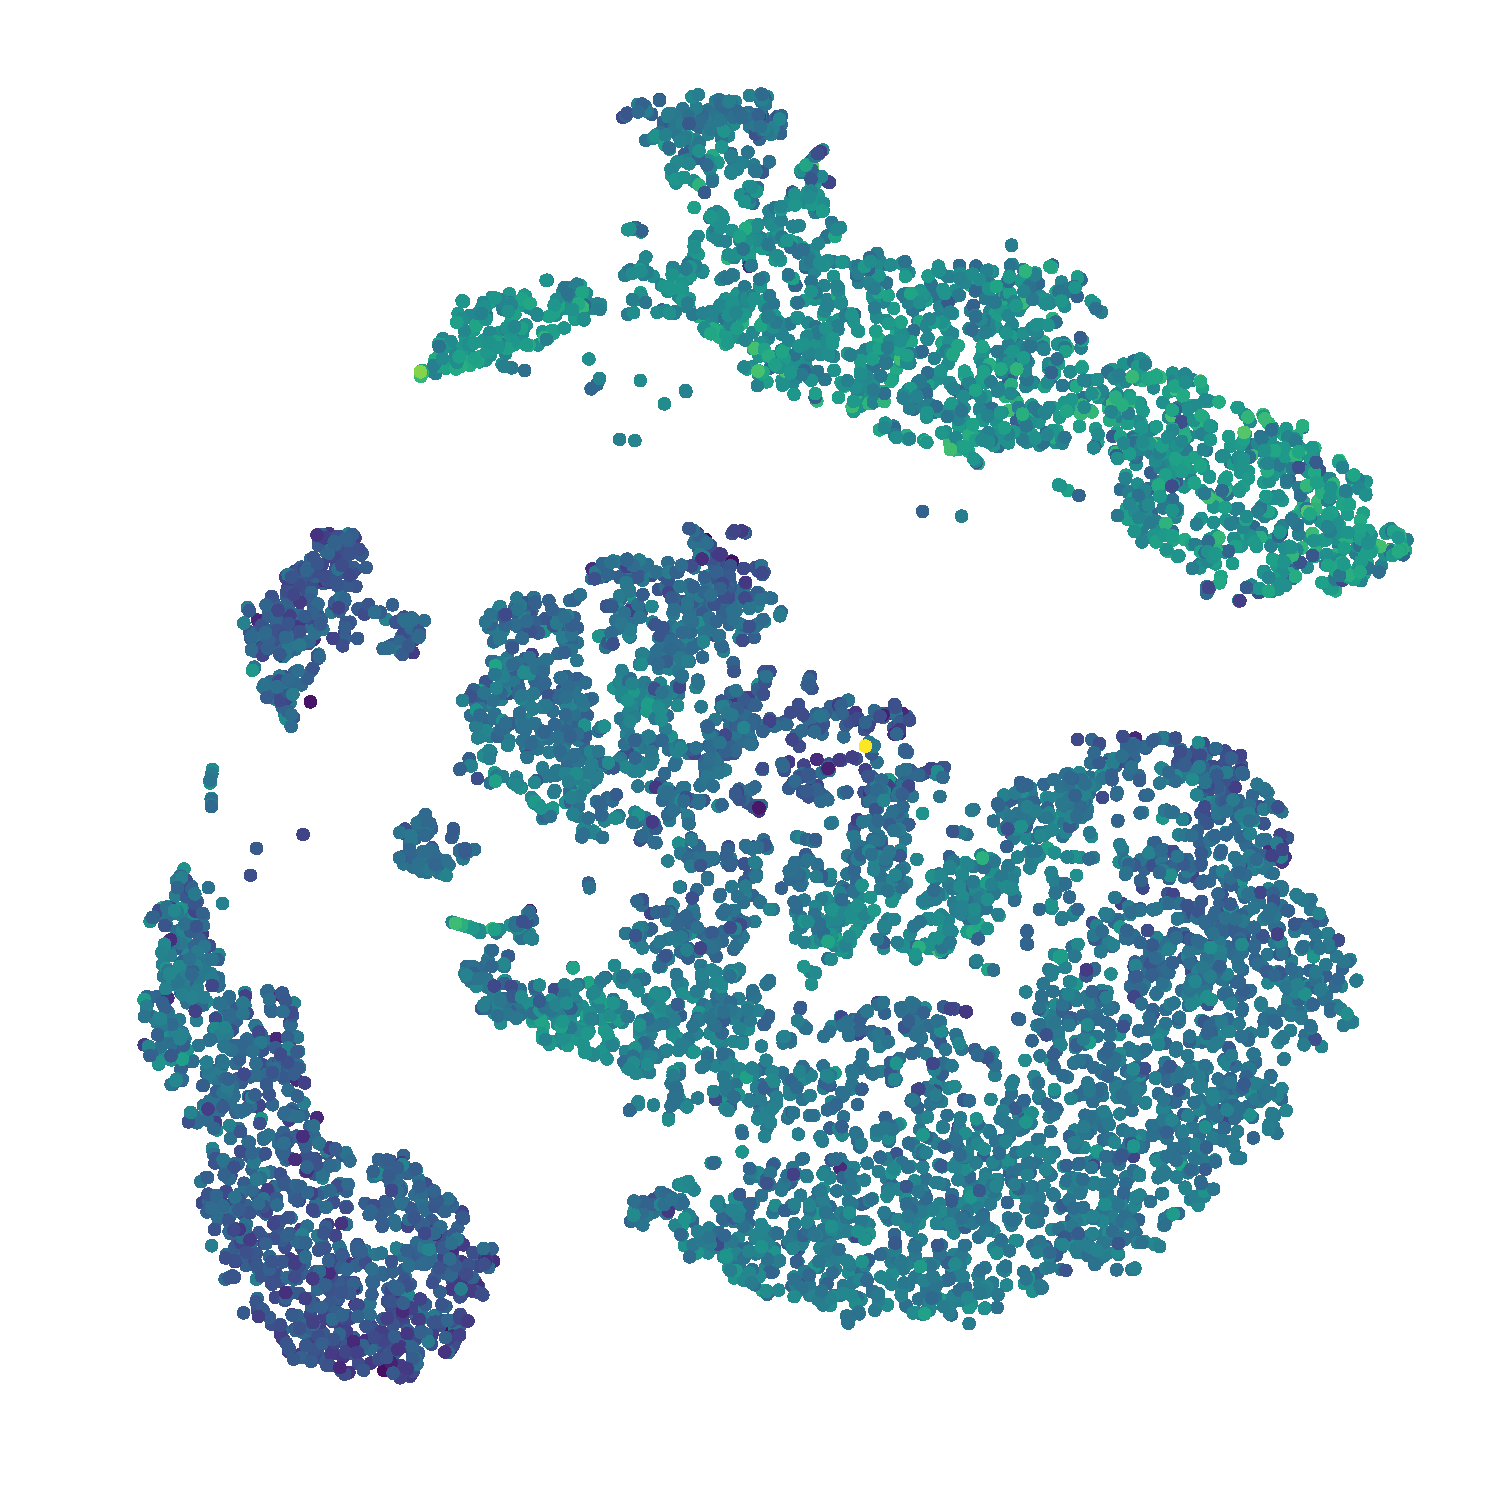
\includegraphics[width=0.7\textwidth]{figures/qc_5.pdf}
        \caption{Embedding of $x$: gene expression data. Each point is a cell. Color is the same quality control metric $s^1$.}
    \end{subfigure}

        \caption[Raw data from the PBMC dataset]{Raw data from the PBMC dataset. $s^1$ is the proportion of transcripts which confidently mapped to a gene for each cell.}
    \label{hsicpbmc}
\end{figure}


We visualize these datasets $x$ and $s$ with tSNE~\cite{Hinton2008} in Figure~\ref{hsicpbmc}. Note that $x$ is correlated with $s$, especially within each cell type. A common application for scRNA-seq is discovering cell types, which can be be done without correcting for the alignment errors~\cite{Wang2017}. A second important application is identifying genes that are more expressed in one cell type than in another---this hypothesis testing problem is called \emph{differential expression}~\cite{deseq2, mast}. Not modeling $s$ can induce a dependence on $x$ which hampers hypothesis testing~\cite{Cole2017}. 

\subsubsection{Deep generative model}

Most research efforts in scRNA-seq methodology research focus on using generalized linear models and two-way ANOVA~\cite{Risso2017,Cole2017} to regress out the effects of quality control metrics. However, this paradigm is incompatible with hypothesis testing. A generative approach, however, would allow marginalizing out the effect of these metrics, which is more aligned with Bayesian principles. Our main contribution is to incorporate these alignment errors into our graphical model to provide a better Bayesian testing procedure. We apply HCV with $Z = \{z, u\}, X=\{x, s\}, \mathcal{Z}_0 = \{z, u\}$. By integrating out $u$ while sampling from the variational posterior, $\int q_\phi(x \mid z, u)dp(u)$, we find a Bayes factor that is not subject to noise.


\begin{figure}[h]
  \centering
  \tikzstyle{latent} = [circle,fill=white,draw=black,inner sep=1pt,
minimum size=30pt, font=\fontsize{15}{15}\selectfont, node distance=1]
\tikzstyle{plate caption} = [caption, node distance=0, inner sep=0pt, font=\fontsize{12}{12}\selectfont,
below left=5pt and 0pt of #1.south east] %

\tikzstyle{second plate caption} = [caption, node distance=0, inner sep=0pt, font=\fontsize{12}{12}\selectfont, below left=5pt and 0pt of #1.south west] %
% \plate [options] {name} {fitlist} {caption} {text}
\renewcommand{\plate}[5][]{ %
  \node[wrap=#3] (#2-wrap) {}; %
  \node[plate caption=#2-wrap] (#2-caption) {#4}; %
  \node[second plate caption=#2-wrap] (#2-caption) {#5}; %
  \node[plate=(#2-wrap)(#2-caption), #1] (#2) {}; %
}


  \newcommand{\ltkiz}{1.5cm}
  
  \scalebox{0.7} {
  \tikz{ %
  \node[obs] (x) {${x}_{ng}$} ; %
  \node[obs, right=2 * \ltkiz of x] (s) {${s}_{nj}$} ; 
  \node[latent, above=0.5 * \ltkiz of x, xshift=\ltkiz] (h) {${h}_{ng}$};
  \node[latent, above=0.5 * \ltkiz of x, xshift=-\ltkiz]  (y) {${y}_{ng}$};
  \node[latent, above=0.5 * \ltkiz of y] (w) {${w}_{ng}$};
    \node[latent, above=0.5 * \ltkiz of w, xshift=-\ltkiz] (l) {${l}_{n}$};
  \node[latent, above=0.5 * \ltkiz of w, xshift=\ltkiz] (z) {${z}_{n}$};
  \node[latent, above=0.5 * \ltkiz of w, xshift=3*\ltkiz] (u) {${u}_{n}$};
  \node[det, above=3* \ltkiz of y, xshift=0*\ltkiz] (t) {$\theta$};
    \node[det, fill=gray!25, above=3* \ltkiz of y, xshift=-1*\ltkiz] (lm) {$l_\mu$};
    \node[det, fill=gray!25, above=3* \ltkiz of y, xshift=-2*\ltkiz] (lv) {$l_\sigma$};

    \plate[inner sep=0.30cm, xshift=-0.cm, yshift=0.cm] {plate1} {(w) (h) (y) (x)} {G} {Genes}; %
    \plate[inner sep=0.30cm, xshift=-0.cm, yshift=0.cm] {plate2} {(s)} {J} {QC};
   \plate[inner sep=0.30cm, xshift=-0.cm, yshift=0.cm] {plate3} {(z) (l) (w) (h) (y) (x) (s) (u) (plate1) (plate2)} {N} {Cells}; %
    \edge {lm} {l};
    \edge {lv} {l};
    \edge {t} {w} ;
    \edge {z} {w} ; %
    \edge {l} {y};
    \edge {h} {x} ; %
    \edge {w} {y}; %
    \edge {y} {x} ; %
    \edge {u} {s};
    \edge {u} {h};
    \edge {u} {w};
  }
  }
\caption[Our proposed modification of the scVI graphical model]{Our proposed modification of the scVI graphical model. Shaded vertices represent observed random variables. Empty vertices represent latent random variables. Shaded diamonds represent constants, set a priori. Empty diamonds represent global variables shared across all genes and cells. Edges signify conditional dependency. Rectangles (``plates'') represent independent replication. }
\label{hsicgraph}
\end{figure}

\paragraph{Generative model}
Our probabilistic model is a modification of the single-cell Variational Inference model~\cite{Lopez292037}. The main difference is the addition of latent variable $u$ and the node for the sequencing errors $s$ (Figure~\ref{hsicgraph}). Let $\ell_\mu, \ell_\sigma \in \mathbb{R}_+^B$ and $\theta \in \mathbb{R}_+^G$. Let $f_w$ (resp. $f_h, f_{\mu_s}$ and $f_{\sigma_s}$) be a neural network with exponential (resp. sigmoid, sigmoid and exponential) link function. Each datapoint $(x_n, s_n)$ is generated according to the following model. First, we draw the latent variables we wish to perform inference over:
\begin{align}
	z_n &\sim \textrm{Normal}(0, I) \\
    u_n &\sim \textrm{Normal}(0, I) \\
    \ell_n &\sim \textrm{LogNormal}(\ell_\mu, \ell_\sigma^2) 
\end{align}

$z$ will encode the biological information, $u$ the technical information from the alignment process and $l$ the sampling intensity. Then, we have some intermediate hidden variables useful for testing and model interpretation that we will integrate out for inference:
\begin{align}
    w_{ng} &\sim \textrm{Gamma}(f_w^g(z_n, u_n), \theta) \\
    y_{ng} &\sim \textrm{Poisson}( \ell_n w_{ng}) \\
    h_{ng} &\sim \textrm{Bernoulli}(f_h^g(u_n)) 
\end{align}

Physically, $w_{ng}$ represents the average proportion of transcripts aligned with gene $g$ in cell $n$. $y_{ng}$ represents one outcome of the sampling process. $h_{ng}$ represents some additional control for the zeros that come from alignment. Finally, the observations fall from:
\begin{align}
    x_{ng} &=
\begin{cases}
y_{ng} & \text{ if } h_{ng} = 0,\\
0 & \text{ otherwise}.
\end{cases} \\
s_{nj} &\sim \textrm{Normal}(f_{\mu_s}^j(u_n), f_{\sigma_s}^j(u_n)) 
\end{align}

where we constrained the mean $f_{\mu_s}^j(u_n)$ to be in the 0-1 range since $s$ is a vector of individual proportions. This model is a very competitive solution for representing single-cell RNA sequencing data.

\paragraph{Variational approximation to the posterior}

Applying AEVB with $X = \{x, s\}, Z = \{z, l, u, w, y, h\}$ seems doomed to fail since some of the variables are discrete. Fortunately, variables $\{w, y, h\}$ can be integrated out analytically: $p(x \mid l, z, u)$ is a Zero-Inflated Negative Binomial distribution. We then apply AEVB with $X = \{x, s\}, Z = \{z, l, u\}$ with the mean-field variational posterior:
\begin{align}
  q_\phi(z, l, u \mid x, s) = q_\phi(z \mid x)q_\phi(l \mid x)q_\phi(u \mid x, s).
\end{align} 

The evidence lower bound is
\begin{equation}
\begin{split}
\log p_\theta(x, s) &\geq \mathbb{E}_{q_\phi(z \mid x)q_\phi(l \mid x)q_\phi(u \mid x, s)}\log p_\theta(x \mid l, z, u) + \mathbb{E}_{q_\phi(u \mid x, s)}\log p_\theta(s \mid u) \\
&- \kld{q_\phi(z \mid x)}{p(z)}- \kld{q_\phi(l \mid x)}{p(l)} - \kld{q_\phi(u \mid x, s)}{p(u)}
\end{split}
\end{equation}

When using the reparametrization trick~\cite{AEVB}, all the resulting quantities can be analytically derived and differentiated. Parameters $\ell_\mu, \ell_\sigma^2$ are set to the mean and average of the number of molecules in all cells of the data (in log-scale). Parameters $\theta$ are learned with variational Bayes, and treated as global variables in the training procedure.

\paragraph{Bayesian hypothesis testing}
We capitalize on our careful modeling to perform principled differential expression. Given two sets of samples $\{x_a \mid a \in A\}$ and $\{x_b \mid b \in B\}$, we would like to test whether a particular gene $g$ is more expressed in population $A$ or in population $B$. 
More formally, for each gene $g$ and a pair of cells $(z_a, u_a)$, $(z_b, u_b)$ with observed gene expression $(x_a, x_b)$ and quality control metrics $(s_a, s_b)$, we can formulate two models of the world under which one of the following hypotheses is true:

$$\mathcal{H}_1^g:= \mathbb{E}f_w^g(z_a, u) > \mathbb{E}f_w^g(z_b, u) \textrm{~~~~vs.~~~~} \mathcal{H}_2^g:=\mathbb{E}f_w^g(z_a, u) \leq \mathbb{E}f_w^g(z_b, u)$$

Where the expectation is taken over $u$ to integrate out the technical variation. Evaluating the likelihood ratio test for whether our datapoints $(x_a, x_b), (s_a, s_b)$ are more probable under the first hypothesis is equivalent to writing a Bayes factor:
\begin{align}
  K = \log_e \frac{p(\mathcal{H}_1^g \mid x_a, x_b)}{p(\mathcal{H}_2^g \mid x_a, x_b)}
\end{align} 

where the posterior of these models can be approximated via the variational distribution:
\begin{align}
  p(\mathcal{H}_1^g \mid x_a, x_b) \approx \mathbb{E}_{\bar{q}} p(f_w^g(z_a, u_a) \leq f_w^g(z_b, u_b) ),
\end{align} 
where $\bar{q} = q(z_a \mid x_a)q(z_b \mid x_b)p(u_a)p(u_b)$. Remarkably, we can use Monte Carlo integration to compute these integrals because all the measures have low dimension.


\paragraph{Dataset} We considered scRNA-seq data from peripheral
blood mononuclear cells (PBMCs) from a healthy donor \cite{Zheng2017}. Our dataset includes 12,039 cells and 3,346 genes, five quality control metrics from CellRanger and cell-type annotations extracted with Seurat~\cite{SEURAT}. We preprocessed the data as in \cite{Lopez292037,Cole2017}. Our ground truth for the hypothesis testing, from microarray studies, is a set of genes that are differentially expressed between human B cells and dendritic cells (n=10 in each group~\cite{Nakaya2011}).

\paragraph{Experiment} 
We compare scVI~\cite{Lopez292037}, a state-of-the-art model, with no observed nuisance variables ($8$ latent dimensions for $z$), and our proposed model with observed quality control metrics. We use five latent dimensions for $z$ and three for $u$. The penalty $\lambda$ is selected through grid search. For each algorithm, we report 1) the coefficient of determination of a linear regression and random forest regressor for the quality metrics predictions based on the latent space, 2) the irreproducible discovery rate (IDR)~\cite{Li2011} model between the Bayes factor of the model and the p-values from the micro-array. The mixture weights, reported in~\cite{Lopez292037}, are similar between the original scVI and our modification (and therefore higher than other mainstream differential expression procedures) and saturate the number of significant genes in this experiment ($\sim$23\%). We also report the correlation of the reproducible mixture as a second-order quality metric for our gene rankings. 

We report our results in Table~\ref{hsicPBMC}. First, the proposed method efficiently removes much correlation with the nuisance variables $s$ in the latent space $z$. Second, the proposed method yields a better ranking of the genes when performing Bayesian hypothesis testing. This is shown by a substantially higher correlation coefficient for the IDR, which indicates the obtained ranking better conforms with the micro-array results. Our denoised latent space is therefore extracting information from the data that is less subject to alignment errors and more biologically interpretable.

\begin{table}[ht]
\centering
\begin{small}
\begin{tabular}{lcccc}
\toprule
      & \multicolumn{2}{c}{\begin{tabular}[c]{@{}c@{}}\textbf{Irreproducible Discovery Rate}\end{tabular}}
      
      %\multirow{2}{*}{\begin{tabular}[c]{@{}c@{}}\vspace{-0.1cm}\\Mixture weights of\\ reproducible genes\end{tabular}} & \multirow{2}{*}{\begin{tabular}[c]{@{}c@{}}\vspace{-0.1cm}\\Rank correlation of\\ reproducible genes\end{tabular}}
      & \multicolumn{2}{c}{\begin{tabular}[c]{@{}c@{}}\textbf{Quality control metrics}\\ \textbf{(coefficient of determination)}\end{tabular}}             \\
                                                                                            & \begin{tabular}[c]{@{}c@{}}\textbf{Mixture}\\\textbf{weight}\end{tabular}    &               \begin{tabular}[c]{@{}c@{}}\textbf{Reproducible}\\ \textbf{correlation}\end{tabular}                                                                                    & \begin{tabular}[c]{@{}c@{}}\textbf{Linear}\\\textbf{Regression}\end{tabular} & \begin{tabular}[c]{@{}c@{}}\textbf{Random Forest}\\ \textbf{Regression}\end{tabular} \\
          \midrule

\textbf{scVI} & \textbf{0.213~$\pm$~0.001} & 0.26~$\pm$~0.07    & 0.195    & 0.129  \\
\textbf{HCV}  & \textbf{0.217~$\pm$~0.003} &\textbf{0.43~$\pm$~0.02}     & \textbf{0.176}    & \textbf{0.123}  \\
\bottomrule
\end{tabular}
\end{small}
\caption[Results on the PBMCs dataset]{Results on the PBMCs dataset. IDR results are averaged over twenty initializations.}
\label{hsicPBMC}
\end{table}
